\subsection{Kafka [SP]}

The straightforward way to store user activity tracking data is to use a logging service.
It collects data, formes batches and stores them in a file system.
However, this approach does not provide a real-time access to stored information.
System that needs to handle real-time data cannot be content with batch-oriented mechanism.
It requires a pipeline that can transfer data between the system components without considerable delays.
Therefore a publish-subscribe mechanism named Kafka was invented by LinkedIn.

Kafka is a message broker that can deliver thousands messages per second. 
It provides high throughput and low latency of data handling.
It is built as a write-ahead log.
Data producers write data into a persistent store and data consumers read these records.
The Kafka structure is illustrated in Figure~\ref{fig:kafka_structure}.

The time of retaining a message is configurable.
The message is kept for a particular period of time, when it is available for consumption.
Then it is removed to free up space.

\begin{figure}[h]
  \centering
  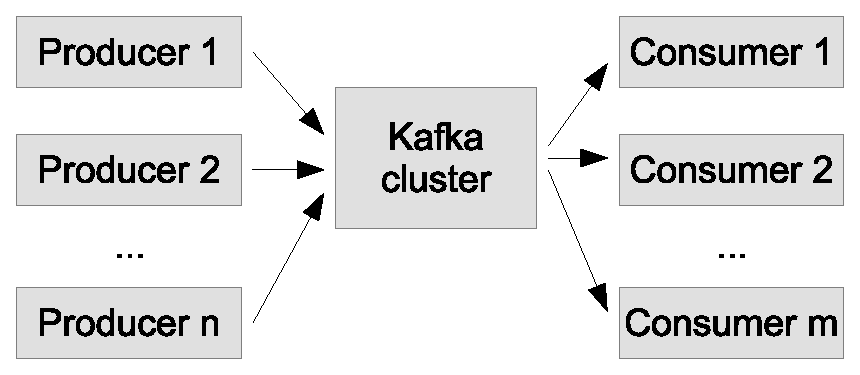
\includegraphics [width=0.5\textwidth]{images/kafka_structure}
  \caption{Kafka structure}
  \label{fig:kafka_structure}
\end{figure} 

\mnote{Kafka topic}
The core abstraction in Kafka is \textit{topic}.
One topic aggregates messages of one type.
For example, the system tracks the user activity, e.g. the number of times he opened a particular application or visited a particular website.
All these records are stored in the topic 'User activity'.
It is recommended to have a small number of topics (no more than a thousand).
However, each topic can contain  billions of messages.

One topic is a log that is spread over a cluster of brokers.
Every Kafka broker consists of zero or more partitions.
Figure~\ref{fig:kafka_topic_structure} illustrates the topic structure.
Kafka continually appends messages to the partitions.
Each partition represents an ordered sequence of messages that are uniquely identified by ids.
This id is called the \textit{offset}.
The sequence of messages is immutable and can only be extended by addition of new messages.
Besides appending, system provides one more operation: messages fetching.
Messages can be obtained from a particular partition, if a beginning message id is specified.
Kafka has an API for these operations, that can be used in different programming languages.

To provide fault tolerance, Kafka replicates each partition across several servers in a Kafka cluster.
One of these servers is a 'leader' and others are 'followers'.
The leader is responsible for handling all read and write requests.
The followers only replicate the leader.
For load balancing each server is simuntaneously a leader and a follower, i.e. for some of its partitions it acts as a leader and for others - as a follower.

The follower acts as a normal consumer, receiving data from the leader and applying it to its log.
Only when all the replicas received the message it is considered to be 'committed' and can be delivered to real consumers.
This guarantees that no message is lost even in the case of the leader failure.
A consumer always receives a message that is committed to the Kafka cluster.
A producer can wait until the message is committed or not, depending on the application logic.

To choose the leader, Kafka maintains a dynamic set of in-sync replicas (ISR).
Only these replicas can participate in the leader elections.
All these nodes must receive a message to consider it to be a committed write.
ZooKeeper stores the ISR set and tracks every change of its membership.
When a Kafka cluster has \textit{n}+1 replicas, it can sustain \textit{n} failures without any problems.

% �������� �������� ��� ��� � ������� ������ ����� ��� ���
%[reference: http://kafka.apache.org/documentation.html]
\begin{figure}[h]
  \centering
  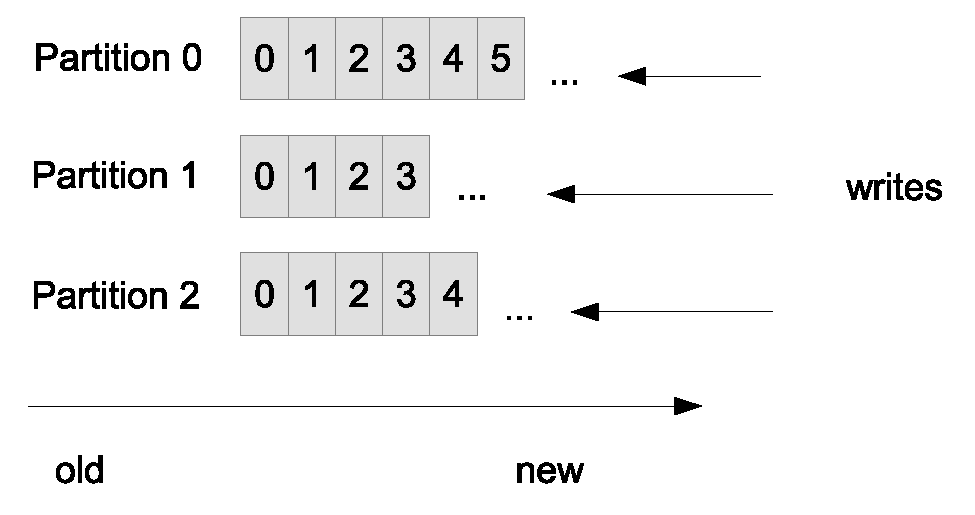
\includegraphics [width=0.5\textwidth]{images/kafka_topic_structure}
  \caption{Kafka topic structure}
  \label{fig:kafka_topic_structure}
\end{figure} 

Kafka uses a publish/subscribe mechanism to establish a communication process between producers and consumers of data.
One subscriber consists of a group of processes that run as a cluster.
Only one machine in this cluster obtains messages from Kafka.
Moreover, it consumes data from a specified partition.
Therefore, the subscriber parallelism depends on the number of partitions of the topic.
Kafka uses ZooKeeper to add or remove nodes from the broker and consumer groups.
It helps to rebalance the load automatically.

The fact that each partition has only one consumer makes it easier to store the metadata about what has been already consumed.
The consumer process just needs to store the last acknowledged message id.
Kafka uses 'at-least-once' semantic for message delivery.
It means that if the cunsumer process crashes, it reprocesses some messages from its partition one more time. 

There are two ways to balance load over Kafka brokers for message producers.
On the one hand, it can be done randomly.
On the other hand, application can supply a key that can be used to hash messages for partitioning.
The latter way guarantees the order of messages between partitions, that is not provided by Kafka.
Also it helps distributed consumers to make in-process aggregation.
In this case a consumer can obtain data from a particular partition, knowing that it contains a part of information it needs.  

For enhancing throughput Kafka introduces three techniques. 
First, it partitions data to production, consumption and brokering parts.
Second, it batches messages to chunks to send them together.
Third, it shrinks the data to decrease the amount of data that should be sent.

\mnote{batching}
The Kafka producer can send messages in synchronous or asynchronous ways.
In asynchronous mode small messages are collected into batches.
This allows to send data in chunks over the network. 
As it is done on application level, it is possible to control the batch size and the maximum time of holding the message.
Kafka allows to group messages from low-volume topics and high-volume topics together, reducing the amount of small requests.
On the filesystem level the mechanism of pagecache is used to buffer writes.
Kafka allows to delay the flush to disk again on the application level.
Similarly, it gives a control over the message boudaries and makes possible to have different policy for different topics.
Batching is also useful on the consumer side.
The client specifies the starting message id and the maximum buffer size it can receive at one time.
Kafka provides a possibility to combine data from several topics in one request.

\mnote{shrinking}
There are two techniques of data shrinking: via serialization and via compression.
Kafka associates schemas with the topics to extract the repeated structure from the messages.
Along with serialization, these schemas can be used to provide the compatibility and integration facilities.
The popular software that is used in combination with Kafka for serialization is Apache Avro.
It is described in details later in this chapter.
Kafka is able to compress several messages into a composite set of messages.
This is done during the batching process of the Kafka producer.
Thus, the messages in the compressed form are transferred to Kafka, where thay are stored and handled also in a compressed form. 

As the data transferred through Kafka is very diverse, a uniform schema is used for every topic.
This schema is kept all the way, from Kafka producer to Kafka consumer.
The schema usage is mandatory and is automatically checked.
As the schema sometimes changes, Kafka stores all its verions.
Each message contains a schema version id with which it was created.
Every schema is thoroughly tested when registered to detect incompatibilities in a timely manner.

\mnote{system monitoring}
A special Kafka topic exists to detect the percentage of data loss.
It audits the number of messages that are sent and received within a given topic over a specified period of time.
For this purpose each producer and consumer periodically notifies the audit topic about the number of processed messages.
The timestamps are extracted from the messages, instead of using the machine time of the message processing.
It is done to deal with delays in message delivering.
Kafka provides a standalone application for monitoring that processes the data from the audit topic.
It computes the ratio of data loss and duplication and is able to produce alert messages.

Kafka can by applied in a number of ways.
First, it can serve as a message broker, allowing to separate data producers from data processing.
Second, it provides facilities for real-time monitoring.
For instance, Kafka can be used to monitor the website users activity or to aggregate some application statistical data.
Third, it can serve as a log aggregation system, that can operate a log messages stream instead of dealing with log files.
This approach decreases latency and makes easier log data collection from several sources.

\mnote{log compaction}
One more Kafka application is a distributed system commit-log, that is used for restoring the failed nodes.
For this purpose Kafka has a specific feature - a \textit{log compaction}.
The main idea of log compaction is that Kafka guarantees that for all the message keys it retains the last known value.
The simpler data retention approaches are time- or size-based.
For example, Kafka removes the log data that is older than a specified period of time.
In this case some values that change rarely can be lost.
On the contrary, log compaction guarantees that at least the last value for each key persists.
This allows to fully restore the state of the broken node.

Another property of log compaction is that it shrinks the log size, removing the old records.
Using the complete log of all changes system can restore its state to any point by re-processing all the changes from the beginning of the log.
However, this approach requires a lot of memory for storing all the changes that leads to poor performance.
Log compaction removes only those records where more recent updates with the same key exist. 
Due to this fact the exterior system does not need to read the whole log and replay all the changes in order to restore its state.
Each topic has its own retention policy, i.e. one cluster can combine time or size retention with log compaction retention.

%[reference: http://kafka.apache.org/documentation.html#majordesignelements]
Figure~\ref{fig:kafka_log_structure} presents the Kafka log structure. 
The head of the log has a sequential numeration (offset) and retains all messages.
The tail of the log has a compacted structure, that contains only selected records.
It is important to mention that the messages in the log tail keep the original offset.
Kafka assignes this offset only once when a message is written for the first time and never changes it.
Moreover, even offsets for removed records are still valid log positions.
In this case Kafka returns the next highest existing value.
For instance, in our case requests with offsets 14, 15, 16 and 17 all return data starting from 17.

\begin{figure}[h]
  \centering
  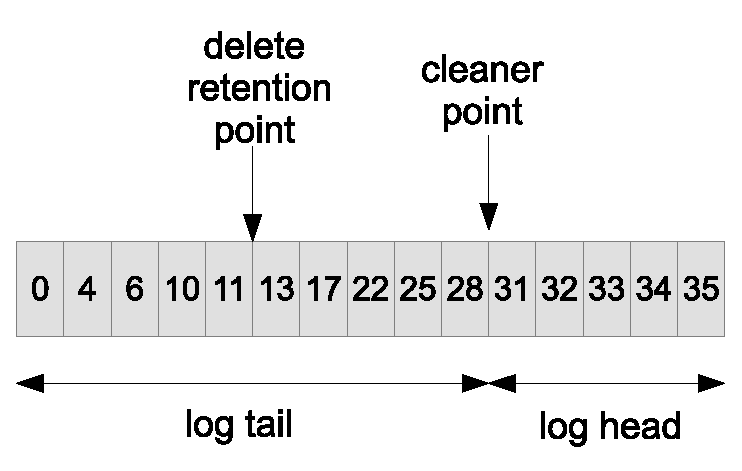
\includegraphics [width=0.5\textwidth]{images/kafka_log_structure}
  \caption{Kafka log structure}
  \label{fig:kafka_log_structure}
\end{figure} 

Compaction also performs message deletions.
If the message is marked to be deleted, all its previous versions (records with the same key) will be removed.
Deletion markers are not retained in the log after 'delete retention point' presented on the picture.

Log compaction is a background process that is run periodically.
Figure~\ref{fig:log_compaction_process} visualises a simple example.
Log compaction process posesses the following properties:
first, it guarantees the messages ordering even after compaction.
Second, the message offset is immutable and serves as a position of the record in the log.
Third, a read operation returns at least the final version for each value associated with a key.

\begin{figure}[h]
  \centering
  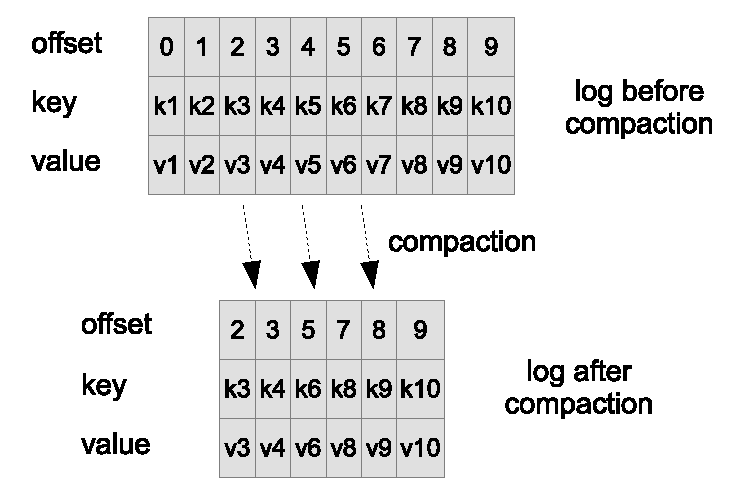
\includegraphics [width=0.6\textwidth]{images/log_compaction_process}
  \caption{Kafka log structure}
  \label{fig:log_compaction_process}
\end{figure} 

The compaction process consists of the following steps:
(1) The log is chosen, that has the biggest number of records from log head to log tail.
(2) For each key in the log head compaction process determines the last offset.
(3) The log is copied from the beginning to the end, removing the keys that occure later in the log. 
   


